%%%%%%%%%%%%%%%%%
% Key table
%%%%%%%%%%%%%%%%%
%http://texblog.net/help/latex/ltx-68.html
\renewcommand{\arraystretch}{1.2}
\begin{table}[!hbt]
\begin{center}

%\begin{tabular*}{0.8\textwidth}{|l|l|}
\begin{tabular}{|l|l|}
\hline 
\textbf{Element} & \textbf{Description}\\
\hline
\raisebox{-3mm}{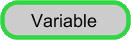
\includegraphics[height=6mm]{ChapterFramework/figures/keybits/variable.jpg}} & Grey boxes are values. Variables change in model runs.\\
\raisebox{-3mm}{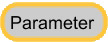
\includegraphics[height=6mm]{ChapterFramework/figures/keybits/parameter.jpg}} & Parameters are fixed for model runs but may change between them\\
\raisebox{-3mm}{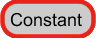
\includegraphics[height=6mm]{ChapterFramework/figures/keybits/constant.jpg}} & Constants do not change\\
\hline
\raisebox{-3mm}{
\includegraphics[height=6mm]{ChapterFramework/figures/keybits/objarray.jpg}} & An array, or set, of objects, such as the set of all firms\\
\hline
\raisebox{-3mm}{
\includegraphics[height=6mm]{ChapterFramework/figures/keybits/ref2obj.jpg}} & For example, a Person may want to keep a reference to their preferred employer\\
\hline
\raisebox{-3mm}{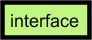
\includegraphics[height=6mm]{ChapterFramework/figures/keybits/interface.jpg}} & A way to provide shared methods to different objects; not important for\\
&understanding model logic, but worth noting where present\\
\hline
\raisebox{-3mm}{
\includegraphics[height=6mm]{ChapterFramework/figures/keybits/method.jpg}} & An object method for achieving a particular model aim\\
\hline
\raisebox{-3mm}{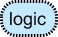
\includegraphics[height=6mm]{ChapterFramework/figures/keybits/logic.jpg}} & Can be one of three things: a logical decision, a calculation\\
& Or an operation on a set (array)\\
\hline
\raisebox{-3mm}{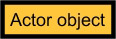
\includegraphics[height=6mm]{ChapterFramework/figures/keybits/actorobj.jpg}} & People or firms\\
\hline
\raisebox{-3mm}{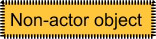
\includegraphics[height=6mm]{ChapterFramework/figures/keybits/nonactorobj.jpg}} & Any other object used in the framework\\
\hline

\end{tabular}

\caption{Key for model diagrams \label{tab:keytable}}
\end{center}
\end{table}